\subsection{Problem 33: Two Masses with Pulley}

\begin{problem}
Two masses, $2m$ kg and $4m$ kg, are attached by a light string. The string is placed over a smooth pulley as shown below. The two masses are at rest before being released and $v$ is the velocity of the larger mass at time $t$ seconds after they are released.

\vspace{0.5em}
\noindent
\begin{center}
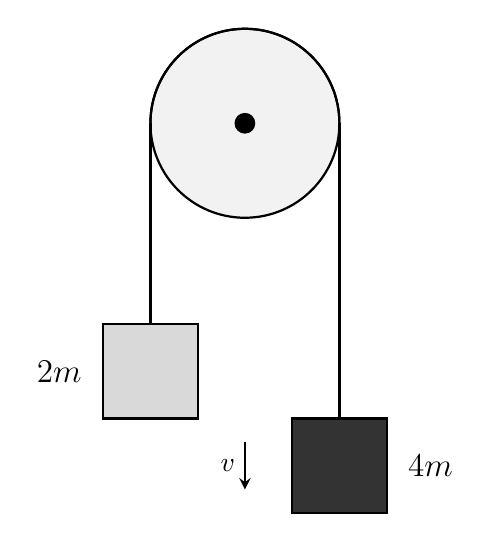
\begin{tikzpicture}[scale=1.5, >=stealth]
    % Pulley wheel
    \draw[thick, fill=gray!10] (0,3) circle (0.8);
    % Pulley axle center dot
    \fill (0,3) circle (2.5pt);
    
    % Ropes (left, right, and arc over pulley)
    \draw[thick] (-0.8, 1.3) -- (-0.8, 3.0);
    \draw[thick] (0.8, 0.5) -- (0.8, 3.0);
    \draw[thick] (-0.8, 3.0) arc (180:0:0.8);
    
    % Left mass (2m)
    \draw[thick, fill=gray!30] (-1.2, 0.5) rectangle (-0.4, 1.3);
    \node[left, font=\large] at (-1.3, 0.9) {$2m$};
    
    % Right mass (4m)
    \draw[thick, fill=black!80] (0.4, -0.3) rectangle (1.2, 0.5);
    \node[right, font=\large] at (1.3, 0.1) {$4m$};
    
    % Velocity vector v of the larger mass
    \draw[->, >=stealth, thick] (0.0, 0.3) -- (0.0, -0.1);
    \node[left] at (0.0, 0.1) {$v$};
\end{tikzpicture}
\end{center}
\vspace{0.3em}

The force due to air resistance on each mass has magnitude $kv$, where $k$ is a positive constant.

\begin{enumerate}
    \item[(i)] Show that
    \[
    \frac{dv}{dt} = \frac{gm - kv}{3m}.
    \]
    
    \item[(ii)] Given that $v < \frac{gm}{k}$, show that when $t = \frac{3m}{k}\ln 2$, the velocity of the larger mass is $\frac{gm}{2k}$.
\end{enumerate}
\end{problem}

\begin{hint}
For part (i), apply Newton's second law to each mass, considering tensions and resistance. For part (ii), solve the differential equation and substitute the given time.
\end{hint}

